% Chapter about Scrum System core

\chapter{Núcleo del Sistema Scrum}

Scrum es un sistema compuesto por la filosofía Scrum (SCRUM Philosophy), como parte del sistema cultural, y tres conjuntos de componentes interrelacionados que forman el "Núcleo del Sistema Scrum"\footnote{El núcleo de Scrum es determinado esencialmente por los organismos y autores que mantienen el scrum originario, o sea los autores (Ken y Jeff) y scrum.org mediante el libro Scrum Guide 2013\cite{Ken-Jeff-2013}.} (ver figura \ref{fig:ScrumSystemCore}). Los tres conjuntos de componentes son: roles, actividades y artefactos. Los roles conforman un sistema de roles que determina las responsabilidades de los actores integrantes, sus relaciones recíprocas, sus restricciones y la relación con los demás componentes. Las actividades conforman la parte principal del sistema de procesos Scrum (Proceso Scrum) que determina las relaciones de organización entre actividades, roles y artefactos. Y los artefactos conforman el conjunto de almacenes o componentes de trabajo. Todo el sistema busca asegurar una cadencia de trabajo que consta de una regularidad basada en iteraciones de tiempo fijo y ceremonias o actividades regulares que permiten la repetibilidad rítmica (predictibilidad del flujo de trabajo) bajo un grado de prestancia.

A continuación se describirán estos componentes y sus relaciones.

\begin{figure}[h]
  \centering
  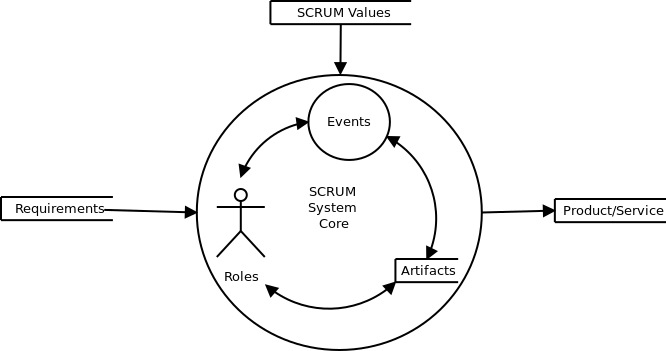
\includegraphics[width=0.99\textwidth]{ScrumSystemCore}
  \caption{Diagrama del Núcleo del Sistema Scrum}
  \centering
  \label{fig:ScrumSystemCore} %\ref{fig:ScrumSystemCore}
\end{figure}


\section{Estructura del Sistema Scrum}

Scrum está pensado como un sistema de trabajo para equipos con tres roles principales: el Product Owner, el Scrum Master y el Development Team. 

Cuando los integrantes del sistema Scrum ejercen los roles mencionados en un flujo de trabajo o proceso Scrum, trabajan sobre tres artefactos esenciales: el Product Backlog (lo que queda por hacer), el Sprint Backlog (lo que se va a hacer) y el Incremento de Producto (lo que logramos hacer). Estos artefactos son tratados en un flujo de trabajo en el cual se construyen productos en forma incremental, en una serie de ciclos cortos de tiempo llamados Sprints. 

En cada ciclo Sprint del flujo de trabajo se practican seis actividades Scrum: refinamiento de producto, planificación, reunión diaria o Daily, desarrollo, revisión de producto y retrospectiva. La actividad de refinamiento de producto (Refinement) no suele tener un nombre unificado; pues, se la suele llamar "Backlog Grooming"\footnote{No se aconseja usar el término Grooming debido a que según el diccionario Oxford English Dictionary tiene connotaciones sexuales.} (aunque no se aconseja usar la palabra grooming), Manteniemiento de Backlog o Refinamiento (Refinement). Salvo el desarrollo, las actividades se consideran reuniones o ceremonias Scrum. El desarrollo no es una reunión Scrum ya que constituye la actividad de producción del producto o servicio. O sea que es donde se produce el incremento de producto.

\section{Sistema de Roles}

El Sistema de Roles (ver figura \ref{fig:ScrumRolesSystem}), en el núcleo de Scrum, es el conjunto de roles y relaciones parte del sistema. Como se mencionó anteriormente, hay tres roles principales: el Product Owner o dueño del producto, el Scrum Master o facilitador y el Equipo de Desarrollo o Equipo a secas (Scrum Development Team, Miembros del Equipo de Desarrollo o Desarrolladores Scrum). También hay roles secundarios como el de Stakeholder, Vendedores y Cuerpo de Asesoramiento de Scrum. El rol Stakeholder es el más importante de los roles secundarios e incluye a los clientes, usuarios y patrocinadores\footnote{\cite{SBOK-2013}}.

Hay que tener en cuenta que este marco contempla solo estos tres roles principales como núcleo en el equipo Scrum y, cuando se implementa en forma ortodoxa, son los únicos roles permitidos. En el caso del Equipo de Desarrollo, cada integrante puede tener diferentes perfiles, características o roles especializados, pero bajo este marco sólo tienen el rol de Desarrollador. Cuando Scrum se integra con otras metodologías o esquemas de roles los desarrolladores pueden cumplir otros roles que funcionan como sub-roles.

\begin{figure}[h]
  \centering
  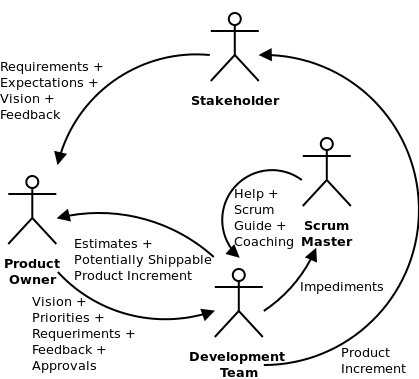
\includegraphics[width=0.80\textwidth]{ScrumRolesSystem}
  \caption{Diagrama del Sistema de Roles Scrum}
  \centering
  \label{fig:ScrumRolesSystem} %\ref{fig:ScrumRolesSystem}
\end{figure}

A continuación se listan los diferentes roles principales:

\subsection{Equipo de Desarrollo}

El Equipo de Desarrollo es parte del Equipo Scrum y son los responsables de construir, o sea desarrollar el producto.
 
Para el cumplimiento del rol Equipo de Desarrollo o desarrollador se deben tener en cuenta las siguientes afirmaciones:

\begin{itemize}
\item Respeta, entiende y sigue los valores ágiles y de Scrum.
\item Crea y gestiona el desarrollo de software comprometiéndose a entregas o fechas de entregas estimadas por el equipo.
\item Es responsable de la calidad técnica del producto.
\item Debe buscar su desarrollo profesional para lograr excelencia técnica. Para ello debe, además, mantener el foco en el aprendizaje, la innovación y el mantenimiento de una actitud de mejora contínua.
\item Debe evitar trabajar en múltiples proyectos teniendo asignación 100\% en el proyecto.
\item Debe priorizar y promover la comunicación cara a cara.
\item Provee estimaciones de ítems de trabajo en forma colaborativa. 
\item Es responsable de gestionar su propio trabajo durante el Sprint.
\item Buscar encontrar una cadencia sostenible para la entrega de incrementos potencialmente entregable de productos.
\item No debe esperar a que le asignen tareas ya que debe seguir la forma "pull" de asignación que consiste en tomar tareas por sí mismo o por consenso de todo el equipo.
\item Monitorea el progreso y el éxito con el resto de los roles del Scrum Team.
\item Debe gestionar los riesgos y problemas junto con los demás roles. En esta vía debe levantar y buscar mitigar los riesgos técnicos.
\item No debe ocultar impedimentos ni información.
\item Debe evitar hacer tareas de otro rol Scrum. En el caso de una implementación ortodoxa no tiene otro rol que el de desarrollador.
\item Debe procurar ser multidisciplinario aprendiendo del conocimientos de los compañeros, aplicando sus habilidades en diferentes tipos de tareas y no especializándose en una sola cosa donde se trabaja en forma estanco (cerrada y hermética).
\item Debe procurar la estabilidad del equipo y su cadencia.
\item Busca mantener el foco en las ceremonias orientados a cumplir los objetivos de la reuniones.
\item Busca mantener el foco en el sprint haciendo que el equipo priorice y trabaje en sólo unos pocos elementos a la vez, acorde a la capacidad del equipo, en lugar de tener muchos trabajos abiertos en paralelo que pueden hacer peligrar el objetivo del sprint.
\item Respeta los acuerdos de trabajo del equipo.
\end{itemize}

\subsection{Product Owner}

El "Product Owner" cumple la función de dueño del producto en el proyecto y es el responsable del negocio. O sea que, es el "Responsable del Producto" o Servicio, quien vela por que el equipo tenga una visión clara y una estrategia, de qué es lo que se va a hacer, para la creación de ese producto o servicio.

Para el cumplimiento del rol PO se deben tener en cuenta las siguientes afirmaciones:

\begin{itemize}
\item Respeta, entiende y sigue los valores ágiles y de Scrum.
\item Debe colaborar con el Scrum Master y con el Equipo de Desarrollo.
\item Es quien busca determinar el mejor producto a conseguir.
\item Es responsable de desarrollar una visión, comunicarla y promoverla.
\item Dirige la estratégica del producto relacionada, entre otras cosas, a la penetración en el mercado, evolución y madurez del producto en el mercado y generación de nuevos mercados.
\item Es responsable del caso de negocio, retorno de la inversión ROI y de los resultados empresariales, evaluando continuamente el impacto en el negocio y buscando maximizar el valor.
\item Es quien provee las "hipótesis requerimientos"\footnote{Bajo el marco Scrum los requerimientos inicialmente constan de hipótesis a ser evaluadas. Son hipótesis porque son dinámicas, no son requerimientos finales sino que son deseos del cliente a ser refinados hasta convertirse en verdaderamente requerimientos.}, por lo que es responsable de entenderlas, escribirlas y transmitirlas en forma eficaz.
\item Es dueño del artefacto Product Backlog y responsable de su orden, priorización y detalle.
\item Es recomendable que esté asignado a un solo Scrum Team con un porcentaje de asignación mayor o igual a un 70 por ciento.
\item Asegura la Colaboración efectiva y la participación de los Stakeholders en el proyecto, administrando sus expectativas y manteniendo una comunicación regular con ellos (representa la voz del cliente).
\item Busca la alineación con otros Product Owners cuando sea necesario desde una perspectiva general de producto, empresa o cliente.
\item Monitorea el progreso y el éxito con el resto de los roles del Scrum Team. 
\item Promueve la gestión del calendario de entregables o mapa de ruta del producto. Es dueño de responder ante el calendario planificado y estimado por el equipo.
\item Busca la satisfacción de los usuarios finales.
\item Ayuda a motivar al equipo para lograr el mejor producto posible.
\item Hace análisis de sistema usando técnicas de modelado para lograr el mejor entendimiento del dominio del problema de negocio e impulsar el diseño del mejor producto posible \footnote{Characteristics of a Great Scrum Team, Barry Overeem, InfoQ, 2016.}.
\item Es hábil para comprender el aspecto operacional del producto.
\item Debe gestionar los riesgos y problemas junto con los demás roles. En esta vía debe levantar y buscar mitigar los riesgos de negocio.
\item No estima, no provee estimaciones ni exige entregas obligadas por fechas.
\item No gestiona el presupuesto de todo el proyecto pero puede gestionar el presupuesto del equipo.
\item No es jefe ni gerente de proyecto.
\end{itemize}

\subsection{Scrum Master}

El Scrum Master es un "Facilitador" y "Coach del Equipo", que es guardián del marco de trabajo Scrum y responsable de mejorar el flujo de valor hacia el cliente. Que sea guardián del marco de trabajo significa que es quien debe asegurar que se siga el sistema Scrum, concientizar sobre la filosofía seguida bajo el mismo, capacitar y entrenar al equipo de desarrollo y facilitar la resolución de impedimentos relacionados a la implementación de Scrum.

Para el cumplimiento del rol SM se deben tener en cuenta las siguientes afirmaciones:

\begin{itemize}
\item Respeta, entiende y sigue los valores ágiles y de Scrum, como también así los fomenta.
\item Es el responsable de que se siga Scrum y brinda apoyo a sus prácticas.
\item Necesita desempeñar su rol con coraje ya que, dentro del equipo, es el principal referente como agente de cambio, movilizador de cambios culturales que pueden ser disruptivos y solucionador de conflictos en busca de facilitar resolver impedimentos.
\item Debe asegurar la gestión de los riesgos y problemas con el equipo. En esta vía debe prestar particular atención a los riesgos relacionados al proceso.
\item Debe buscar remover obstáculos e impedimentos.
\item Es responsable de buscar lograr la mejora continua del proceso o sistema de trabajo.
\item Busca conseguir que se haga el trabajo y que se logren lo objetivos.
\item La mejor manera de cumplir el rol es estar tiempo completo en este rol (asignación 100 por ciento).
\item Sirve de embajador del equipo ante la organización, obrando en ocasiones como mensajero, representante o interfaz.
\item Debe ser guardián del equipo protegiéndolo de perturbaciones negativas externas.
\item Monitorea el progreso y el éxito con el resto de los roles del Scrum Team.
\item Ayuda al Equipo a encontrar una cadencia sostenible (con ritmo y naturalidad) para la entrega de incrementos potencialmente entregable de productos. 
\item Busca lograr un entorno seguro y de apoyo que genere confianza y respeto mutuo (seguridad psicológica). Ayuda a lidiar con los conflictos personales.
\item Busca establecer acuerdos claros y que se cumpla lo pactado.
\item Es un líder servicial cuyo enfoque se centra en las necesidades de los miembros del equipo, con el objetivo de lograr resultados alineados con los valores, principios y objetivos planteados.
\item Es un entrenador y mentor de los miembros del equipo con un enfoque en la cultura, mentalidad y el comportamiento.
\item Facilita la resolución de conflictos para abordar actitudes proactivas, productivas y colaborativas.
\item Facilita el aprendizaje de Scrum, agilidad, técnicas y métodos complementarios relevantes para facilitar el proceso de trabajo.
\item Considera diferentes formas de trabajar con el equipo Scrum buscando aplicar las más adecuadas según el contexto.
\item Busca comprender la esencia de la comunicación en los diálogos del equipo Scrum y ayudar a concretar sus acciones y su entendimiento.
\item La presencia en la Daily Scrum no es obligatoria, pero es aconsejable que esté para facilitarla y moderarla cuando sea necesario.
\item Asegura el cumplimiento de los time-box facilitando la adopción de disciplina por parte del equipo.
\item Procura lograr un equipo motivado.
\item Un gran Maestro Scrum es un agente de cambio entendiendo que algunos cambios sólo se producirán si se es disruptivo. Está preparado para ser lo suficientemente disruptivo como para promover un cambio dentro de la organización\footnote{Characteristics of a Great Scrum Team, Barry Overeem, InfoQ, 2016.}.
\item Comprende sobre el aspecto técnico del desarrollo manejando diferentes técnicas y prácticas de desarrollo. En el caso de desarrollo de software sabe de ingeniería de software.
\item No debe estimar junto al Equipo de Desarrollo ni hacer tareas de otro rol como, por ejemplo, desarrollar (programar, probar, etc.).
\item No es jefe, no es gerente de proyecto, no debe gestionar al Equipo de Desarrollo y no es responsable por la planificación del proyecto.
\item No asigna tareas, sino que procura que el equipo se las auto-asigne o las tome por voluntad propia y auto-organización.
\end{itemize}

Se puede ver un resumen del foco de las responsabilidades de los roles en la figura \ref{fig:ScrumRolesResponsibility}.

\begin{figure}
  \centering
  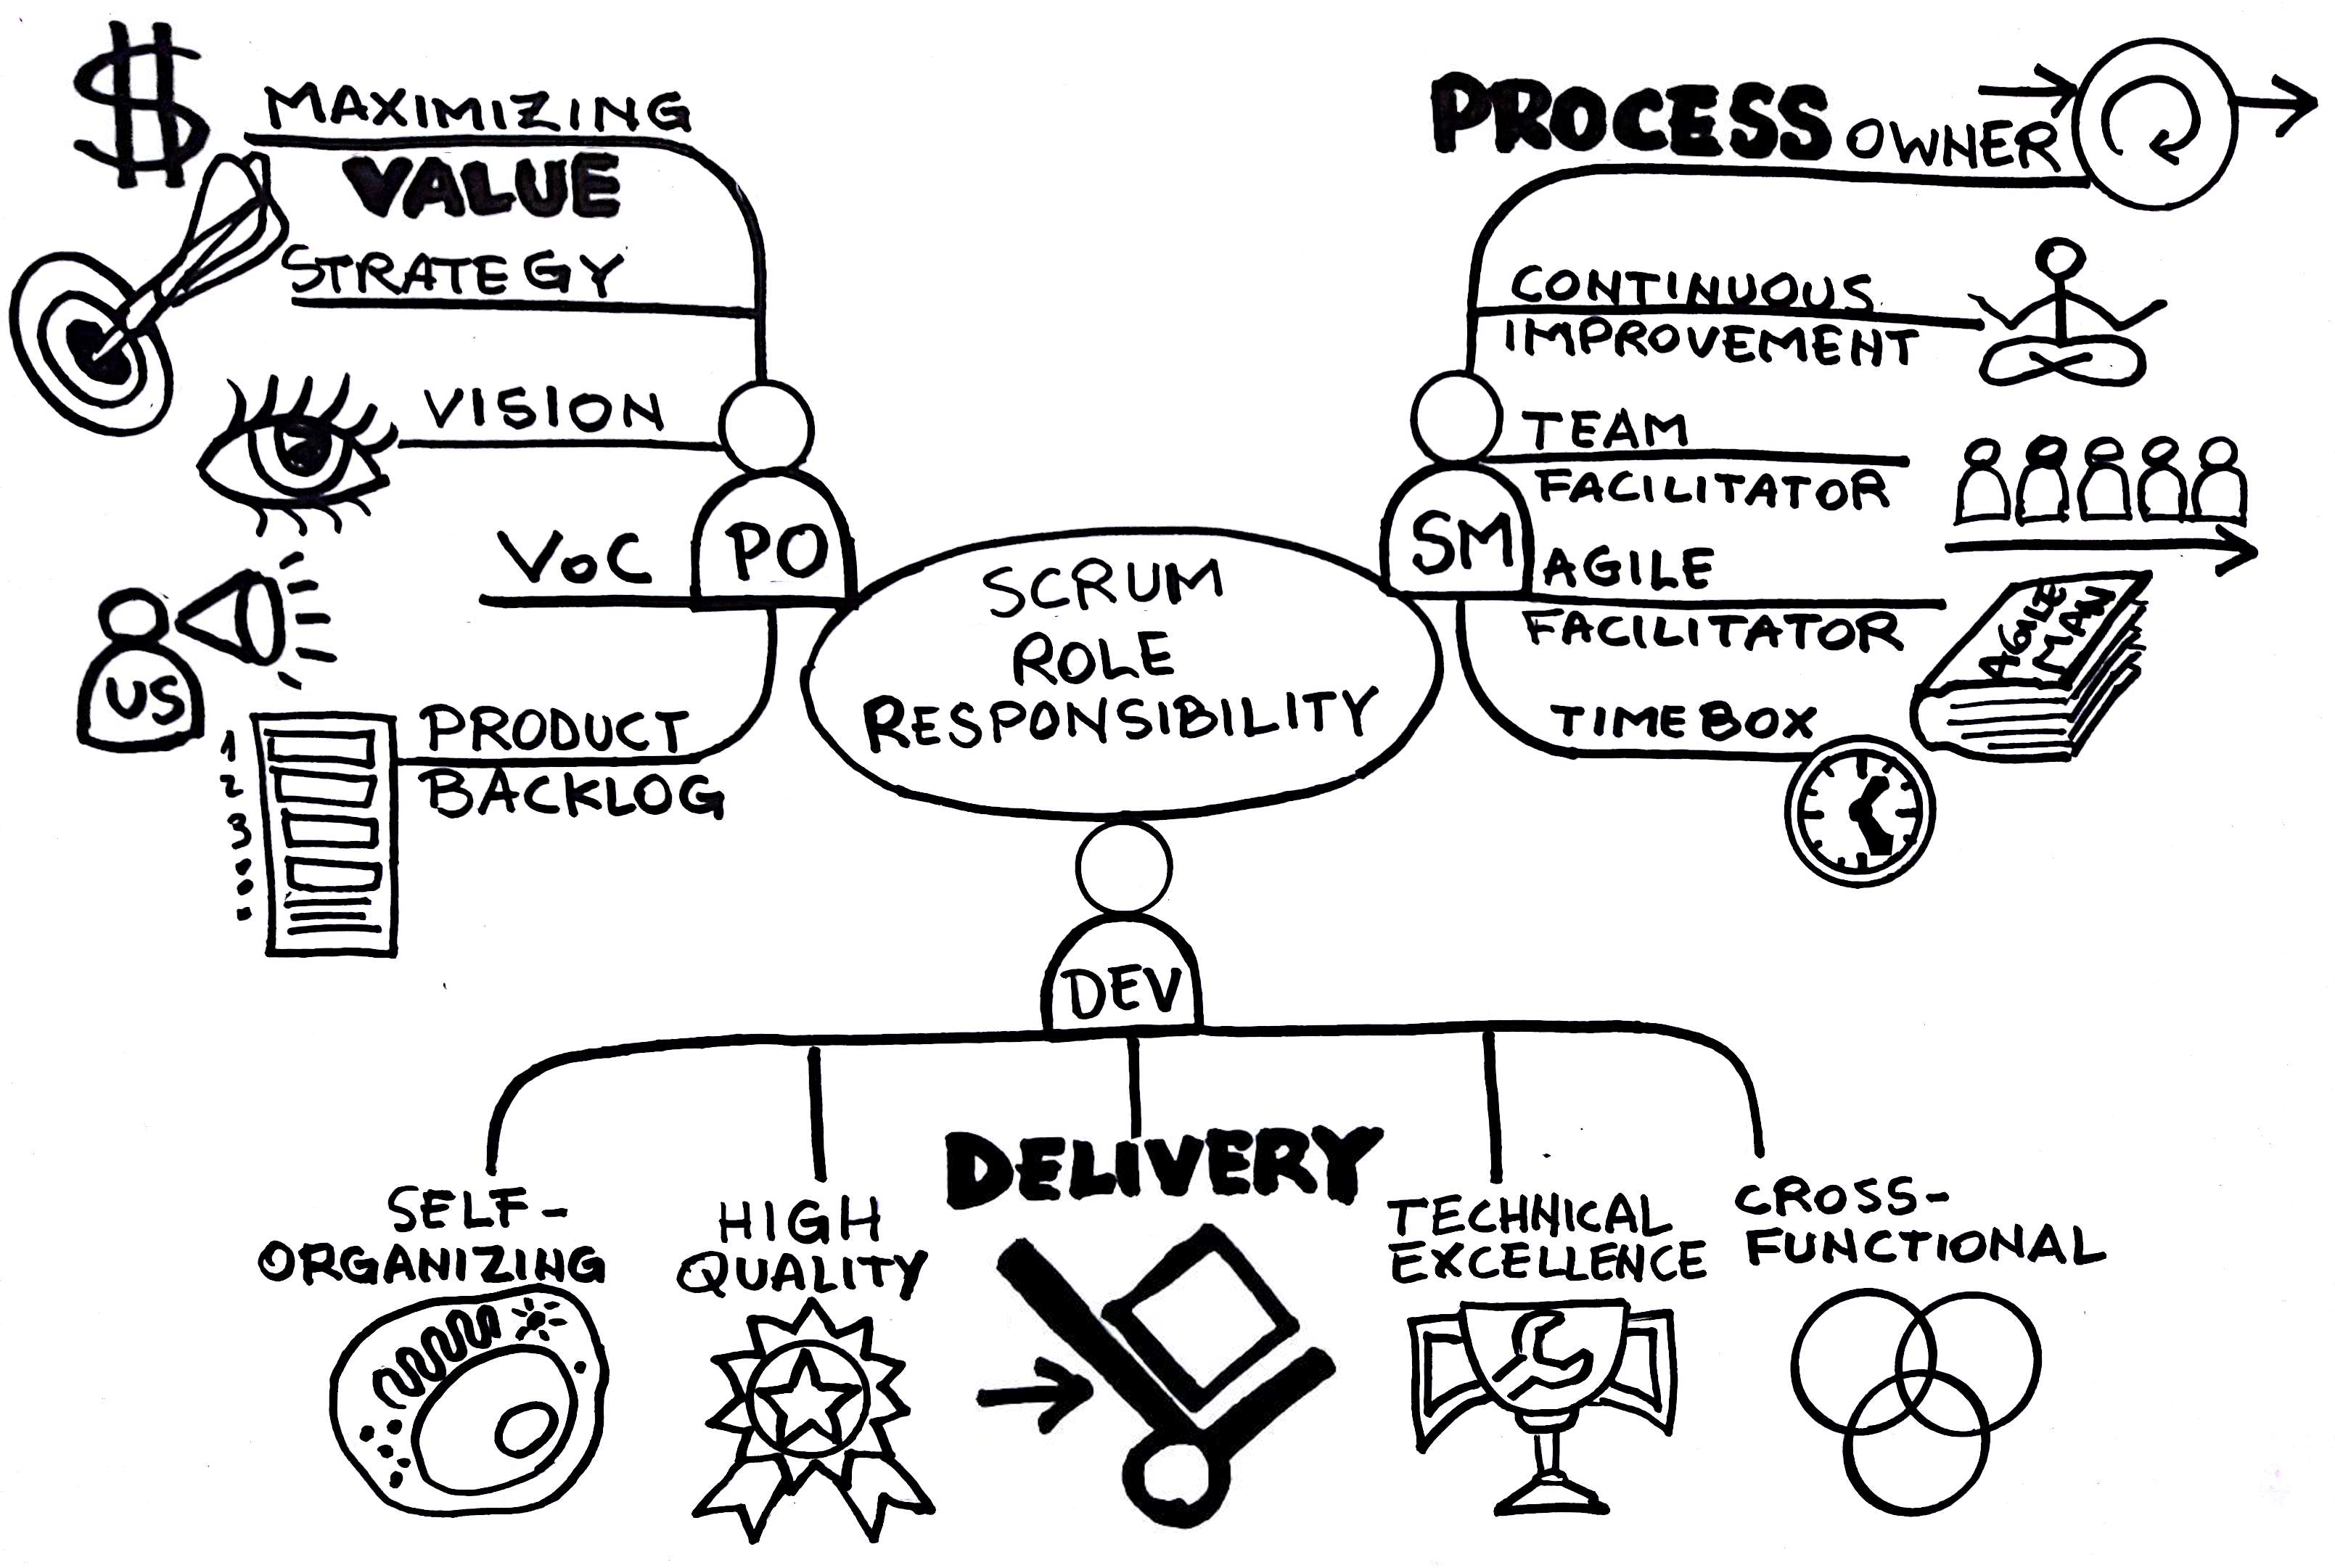
\includegraphics[width=0.95\textwidth]{ScrumRolesResponsibility}
  \caption{Mapa mental resumen didáctico del foco según las responsabilidades de los roles.} El PO se focaliza en maximizar el valor, la estrategia de negocio, la visión y la voz del cliente. El equipo de desarrollo (DEV) se responsabiliza principalmente de la entrega ágil, su auto-organización, la alta calidad técnica (excelencia técnica) y su multidisciplinariedad (trabajo colaborativo no especializado). El SM es dueño del proceso, por lo que se focaliza en el proceso de trabajo e ingeniería, la mejora continua, el trabajo en equipo y la facilitación ágil (referente ágil y de scrum).
  \centering
  \label{fig:ScrumRolesResponsibility} %\ref{fig:ScrumRolesResponsibility}
\end{figure}


\section{Proceso Scrum}

En el proceso Scrum o sistema de flujo de actividades Scrum (ver figura \ref{fig:ScrumFlow}) los miembros del equipo Scrum colaboran para crear una serie de Incrementos de Producto durante iteraciones de intervalos fijos de tiempo denominados Sprints. En cada iteración Sprint, se comienza por una Planificación del Sprint para producir un Backlog del Sprint a partir del Backlog de Producto, es decir un plan para el Sprint. El equipo se auto-organiza para realizar el Desarrollo, mediante reuniones Diarias de Scrum para coordinar y asegurarse de estar produciendo el mejor Incremento de Producto posible en el proceso de desarrollo del producto o servicio. Cada incremento satisface el criterio de aceptación del Product Owner y la Definición de Hecho o "Definition of Done" compartida por el equipo para satisfacer el criterio de tarea terminada. Junto al proceso de desarrollo se hace también un Refinamiento del Backlog ("Refinement") para prepararse para la reunión de planificación del próximo Sprint. Finalizando cada ciclo se termina el Sprint con una reunión de Revisión del Sprint y luego una reunión Retrospectiva del Sprint, revisando el producto y su proceso con una perspectiva crítica y de mejora contínua. 

\begin{figure}[h]
  \centering
  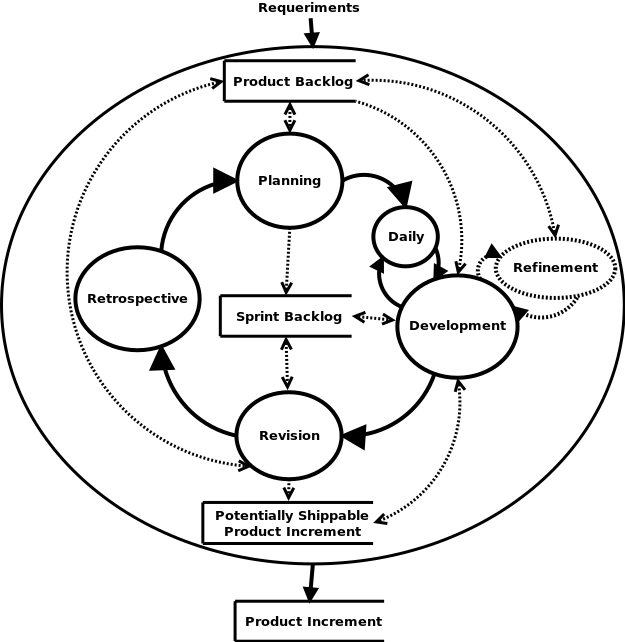
\includegraphics[width=0.99\textwidth]{ScrumFlow}
  \caption{Diagrama de Flujo de Datos del Proceso Scrum}
  \centering
  \label{fig:ScrumFlow} %\ref{fig:ScrumFlow}
\end{figure}

\subsection{Reuniones principales}

\begin{itemize}

\item \textbf{Planificación:} es una actividad o una conversación de duración fija al principio de cada Sprint para decidir sobre lo que se terminará y se demostrará en la revisión.

Esta reunión se divide generalmente en tres partes principales: una primera parte es estratégica relacionada al "qué", una segunda parte táctica relacionada al "cómo" y una tercera relacionada al acuerdo de cierre. 

\begin{itemize}

\item \textbf{Planificación relacionada al "Qué":} La primera parte se propone responder a: ¿Qué trabajo será realizado? En esta parte se desarrolla la definición de lo que se necesita hacer, de cuáles hipótesis del Cliente se desean desarrollar. En este proceso se crean los ítems de Product Backlog o PBIs y los Criterio de Aceptación. Los PBIs son generalmente escritos por el PO y están diseñados para asegurar que las hipótesis de requisitos del Cliente estén claramente representadas y puedan ser plenamente comprendidas por todos los Stakeholders y los desarrolladores del equipo.
En la dinámica de la reunión, el PO cuenta cuáles son los PBIs disponibles que pasan el criterio de completitud o DoR (una definición de listo o refinado), para ser desarrollados en el Sprint y los explica para que sean comprendidos por el Equipo. Mientras sucede esto los integrantes del equipo hacen todas las preguntas que consideren necesarias para comprender los detalles de lo que se desea realizar y puedan, así, entregar una estimación del trabajo a comprometer. Luego de estimar se procede a una negociación entre el PO y el Equipo de cuáles son los PBIs que el Equipo se compromete a desarrollar para transformar en un incremento de producto potencialmente entregable. En este proceso el SM se encarga de facilitar la ceremonia, moderar y tratar de asegurar de que todos los Stakeholder del proyecto que sean necesarios para para aclarar detalles estén presentes o sean contactados para hacer las respectivas aclaraciones.
El resultado de este proceso es un conjunto de PBIs estimados y comprometidos inicialmente para ser trabajados en el Sprint.

\item \textbf{Planificación relacionada al "Cómo":} En la segunda parte de la planificación se propone responder a: ¿Cómo será realizado el trabajo? Esta parte es táctica y por lo tanto más técnica por lo que no es necesaria la presencia del Product Owner, pero debe estar disponible para contestar preguntas y clarificar dudas surgidas sobre la marcha. En esta reunión el Equipo discute cómo implementará los PBIs, diseñando inicialmente, en forma general y abstracta (acuerdo de alto nivel), las soluciones y definiendo tareas implicadas. 

\item \textbf{Cierre de planificación como "Acuerdo":} Cuando termina la reunión relacionada al "Cómo", el Equipo debe negociar y comprometer finalmente el alcance del Sprint formando un acuerdo de compromiso con el Product Owner. El resultado de este proceso es un conjunto de PBIs que forman el alcance del Sprint, o sea el Sprint Backlog, el objetivo del Sprint y una visión de diseño o arquitectura a alto nivel de lo que se desea implementar junto con un conjunto de tareas planificadas para el Sprint.

\end{itemize}

\item \textbf{Scrum Diario:} la Daily Scrum o Stand-up meeting es una actividad o una reunión diaria obligatoria del Equipo Scrum, en el lugar de trabajo, con una duración fija, que sirve para coordinación y organización mediante una retroalimentación del estado de actividades de cada integrante del Equipo. Permite identificar impedimentos bloqueantes, actualizar artefactos, revisar el Sprint Backlog, ayudar a disminuir riesgos e identificar personas que pueden servir de ayuda a determinadas tareas. En esta reunión los miembros del equipo se reúnen, de pie, para informar de sus progresos en el Sprint y planificar las actividades del día. Para ello proporcionan respuestas a tres preguntas:

\begin{itemize}
\item{¿Qué hice ayer?}
\item{¿Qué voy a hacer hoy?}
\item{Si tengo obstáculos: ¿Qué impedimentos tengo?}
\end{itemize}

Es obligatorio que el Equipo asista a esta reunión y es aconsejable que esté el SM para facilitarla y servir de moderador. El PO puede asistir también para seguir el avance del trabajo durante la iteración, pero puede participar como oyente o no asistir. Sin embargo, si se quiere lograr un mejor trabajo de equipo y mayor integración con el PO, es aconsejable que siga la dinámica al igual que el Equipo.

\item \textbf{Refinamiento:} es una actividad o reunión para refinar la lista de PBIs o Product Backlog que consiste en trabajar sobre las hipótesis de requerimientos, definirlas y añadirles detalles, granularizarlas, estimarlas y priorizarlas. Es un proceso continuo que hace el Product Owner, pero formalmente como reunión se desarrolla con participación del Equipo en colaboración para examinar y revisar los elementos del Product Backlog. En esta reunión la responsabilidad recae en el PO y el Equipo solo colabora.

En la reunión que se hace con el equipo se desarrollan las siguientes actividades:
  \begin{itemize}
  \item{El PO presenta los próximos ítems de backlog al equipo.}
  \item{Se conversa grupalmente aspectos sobre ítems de backlog: }
    \begin{itemize}
    \item{Conversación, entendimiento y ajuste.}
    \item{Búsqueda de posibilidad de granularización.}
    \item{Identificación de dependencias.}
    \item{Detección de riesgos que pueden hacer que esas historias no se completen e identificación de actividades a realizar para mitigarlos.}
    \end{itemize}
  \item{Estimación.}
  \item{Priorización.}
  \end{itemize}

\item \textbf{Revisión:} es una actividad o una conversación de duración fija al final de cada Sprint para dar retroalimentación sobre el avance del producto. En esta reunión se evalúa el incremento funcional potencialmente entregable construido por el Equipo en el proceso de desarrollo. Para lograr hacer esto el Equipo de Desarrollo junto al PO y los Stakeholder involucrados, revisan los resultados funcionales y operativos (producto utilizable) del Sprint. El objetivo es recibir una retroalimentación de lo construido y aprobar o rechazar los PBIs que pasaron la DoD y son potencialmente entregables, para lo que los Stakeholder prueban el producto construido y proveen su feedback. En este proceso pueden haber cambios o nuevas hipótesis de requisitos que surjan para agregarse en el Product Backlog.

\item \textbf{Retrospectiva:} es una actividad o una conversación de duración fija al final de cada Sprint para que el Equipo reflexione y busque mejoras procedimentales. En esta reunión se intentan responder tres preguntas relacionadas al "proceso": ¿qué se hizo mal?; ¿qué se hizo bien? y ¿que se puede mejorar?
De esta reunión deberían quedar lecciones aprendidas y un listado de acciones a tomar para mejorar la forma de trabajar. Las acciones a tomar deben ser desarrolladas en el siguiente Sprint y analizadas en la retrospectiva del mismo.
En esta reunión es obligatoria la asistencia del Equipo con el SM y la asistencia del PO es optativa, sin embargo, podría asistir si el equipo lo considera apropiado \footnote{\cite{Martin-Alaimo-2014}}.

\end{itemize}

\section{Flujo de artefactos}

Los artefactos ítems de trabajo fluyen desde que se definen en el Backlog de Producto hasta que se transforman en incremento de producto. Los ítems de trabajo son items de valor para el cliente que comienzan su nacimiento como ítems de backlog o PBIs del Backlog de Producto. Debido a que el dueño del Backlog de Producto es el Product Owner, es él quien crea los PBIs, ya sea por trabajo individual o con la colaboración del Equipo de Desarrollo. Los PBIs son requerimientos que puede escribirse de diferente manera. Es común escribir los PBIs en forma de Historias de Usuario \cite{Cohn-2004}, pero no es un requisito de Scrum. Estos PBIs son refinados por la actividad de Refinamiento de Backlog hecha por el PO y el Equipo de Desarrollo mientras se practica el desarrollo de un Sprint y son priorizados por el ProductOwner. En la reunión de planificación "Planning" se toman PBIs que cumplan el criterio de aceptación o "Definition of Ready" (2 "Selection") para ser incluidos en el "Sprint Backlog" y el Equipo de Desarrollo pueda trabajar en ellos en el Sprint. A medida que el Equipo de Desarrollo termina un ítem "Sprint Backlog" cumpliendo el criterio de aceptación "Definition of Done" (3 "increment") se genera un Incremento de Producto candidato potencialmente entregable (Potentially Shippable Product Increment). Luego en la Revisión se acepta el Incremento de Producto candidato pasando a ser efectivamente un Incremento de Producto listo para ser entregado o desplegado, para "Release" (4 "releasing"). En caso de no ser aprobado (5 "Rejection") pasa nuevamente al Product Backlog para ser tenido en cuenta en el próximo Sprint. Los ítems de "Sprint Backlog" que no se lograron terminar también vuelven (6 "comeback") al "Product Backlog". Esto ocurre formalmente en la revisión \cite{Martin-Alaimo-2014}.

\begin{figure}[h]
  \centering
  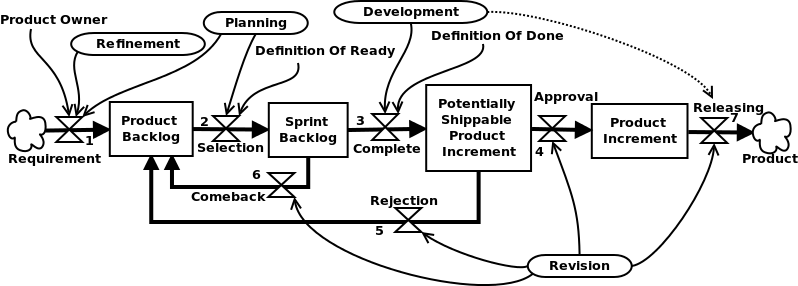
\includegraphics[width=0.99\textwidth]{ScrumArtifactsStockFlow}
  \caption{Diagrama de Flujo de Stock de artefactos Scrum}
  \centering
  \label{fig:ScrumArtifactsStockFlow} 
\end{figure}

\subsection{Definición de preparado}

La definición de preparado, "Definition of Ready" o DoR es un tipo de Definición de Terminado particular (previo al desarrollo) que se corresponde con las condiciones para que un PBI pueda pasar a formar parte de un Sprint Backlog. Si un PBI no cumple con su DoR no puede ser tomado en una planificación para ser ítem de trabajo del Sprint planeado, ya que es un ítem que no está suficientemente preparado para ser comprometido para el desarrollo. O sea que, la definición de preparado permite entonces tener un punto de acuerdo entre el PO y el Equipo, permitiendo conocer cuándo una historia de usuario está realmente lista para evaluar su factibilidad de desarrollo en una reunión de planeamiento y ser llevada a un Sprint.

Un ejemplo de DoR puede ser el que sigue:

\begin{enumerate}
\item{Historia de usuario definida.}
\item{Cumple el criterio INVEST (INVEST es tratado posteriormente).}
\item{Hay un contexto de negocio claro.}
\item{Criterios de aceptación definidos, claros y comprobables.}
\item{Identificación de dependencias con otras historias de usuario.}
\item{Hay una idea clara de cómo se puede demostrar la historia en una review.}
\item{El equipo tiene el conocimiento para analizarla.}
\end{enumerate}

\subsection{Definición de Terminado}

Los ítems de artefactos fluyen por sus diferentes estados (o Stock en el flujo de Stock) a medida que cumplen con determinadas condiciones de cambio de estado. A estas condiciones que deben cumplir para cambiar de estado se las llama definición de terminado y funcionan como válvulas para que los ítems pasen de un Stock a otro Stock. Por ejemplo para que un ítem pase del Stock de Sprint Backlog a Incremento de Producto Potencialmente Entregable debe cumplir una definición de terminado, "Definition of Done" o DoD. Normalmente se suele considerar que el DoD es una lista de actividades que cada elemento de trabajo debe completar para poder ser considerado potencialmente entregable para un cliente dado y conforma un "entendimiento compartido de lo que significa que el trabajo esté completado"\footnote{\cite{Ken-Jeff-2013}}.

\section{Reglas y Consideraciones}

Además se establecen alguna consideraciones relacionadas a tiempos y tamaños. Se aconseja un tamaño de equipo de desarrollo mayor a 4 miembros y menor a diez (7 +- 2), o sea entre cinco y nueve (ver figura \ref{fig:TeamSize_by_Lawrence_Putnam})\footnote{El estudio de Lawrence Putnam sigiere 7 miembros de equipo óptimo con más o menos dos personas (2013). Algunos estudios dicen que el equipo debe rondar las 8 a 10 personas (Emery and Emery 1975, Bayer and Highsrriith 1994).}. Por debajo de este número mínimo se tiene un equipo pobre que puede brindar un producto pobre y por sobre ese número máximo se aumenta la complejidad de gestión y coordinación del equipo disminuyendo el funcionamiento apropiado tras la metodología planteada. También se recomienda una duración de Sprint no mayor a un mes \cite{Ken-Jeff-2013}. La Reunión de Planificación de Sprint debería tener un máximo de duración de ocho horas para un Sprint de un mes. El Scrum Diario o "daily" es una reunión con un bloque de tiempo de 15 minutos para que el Equipo de Desarrollo sincronice sus actividades y cree un plan para el día. Por ejemplo, una daily mayor de 15 minutos se puede considerar larga y en 15 minutos es complicado que más de 15 personas puedan exponer lo que hicieron, lo que harán y si tienen bloqueos. Por eso se aconseja, como máximo, nueve personas en el equiopo de desarrollo. En lo que concierne a la Revisión, el tiempo estipulado es de cuatro horas para Sprints de un mes o dos horas para uno de una quincena. La reunión de Retrospectiva  debería estar restringida a un bloque de tiempo de tres horas para Sprints de un mes o  a una hora y media para los de una quincena. Las reuniones de Planificación, Revisión y Retrospectiva deberían ser proporcionales a la duración del Sprint.

\begin{figure}[h]
  \centering
  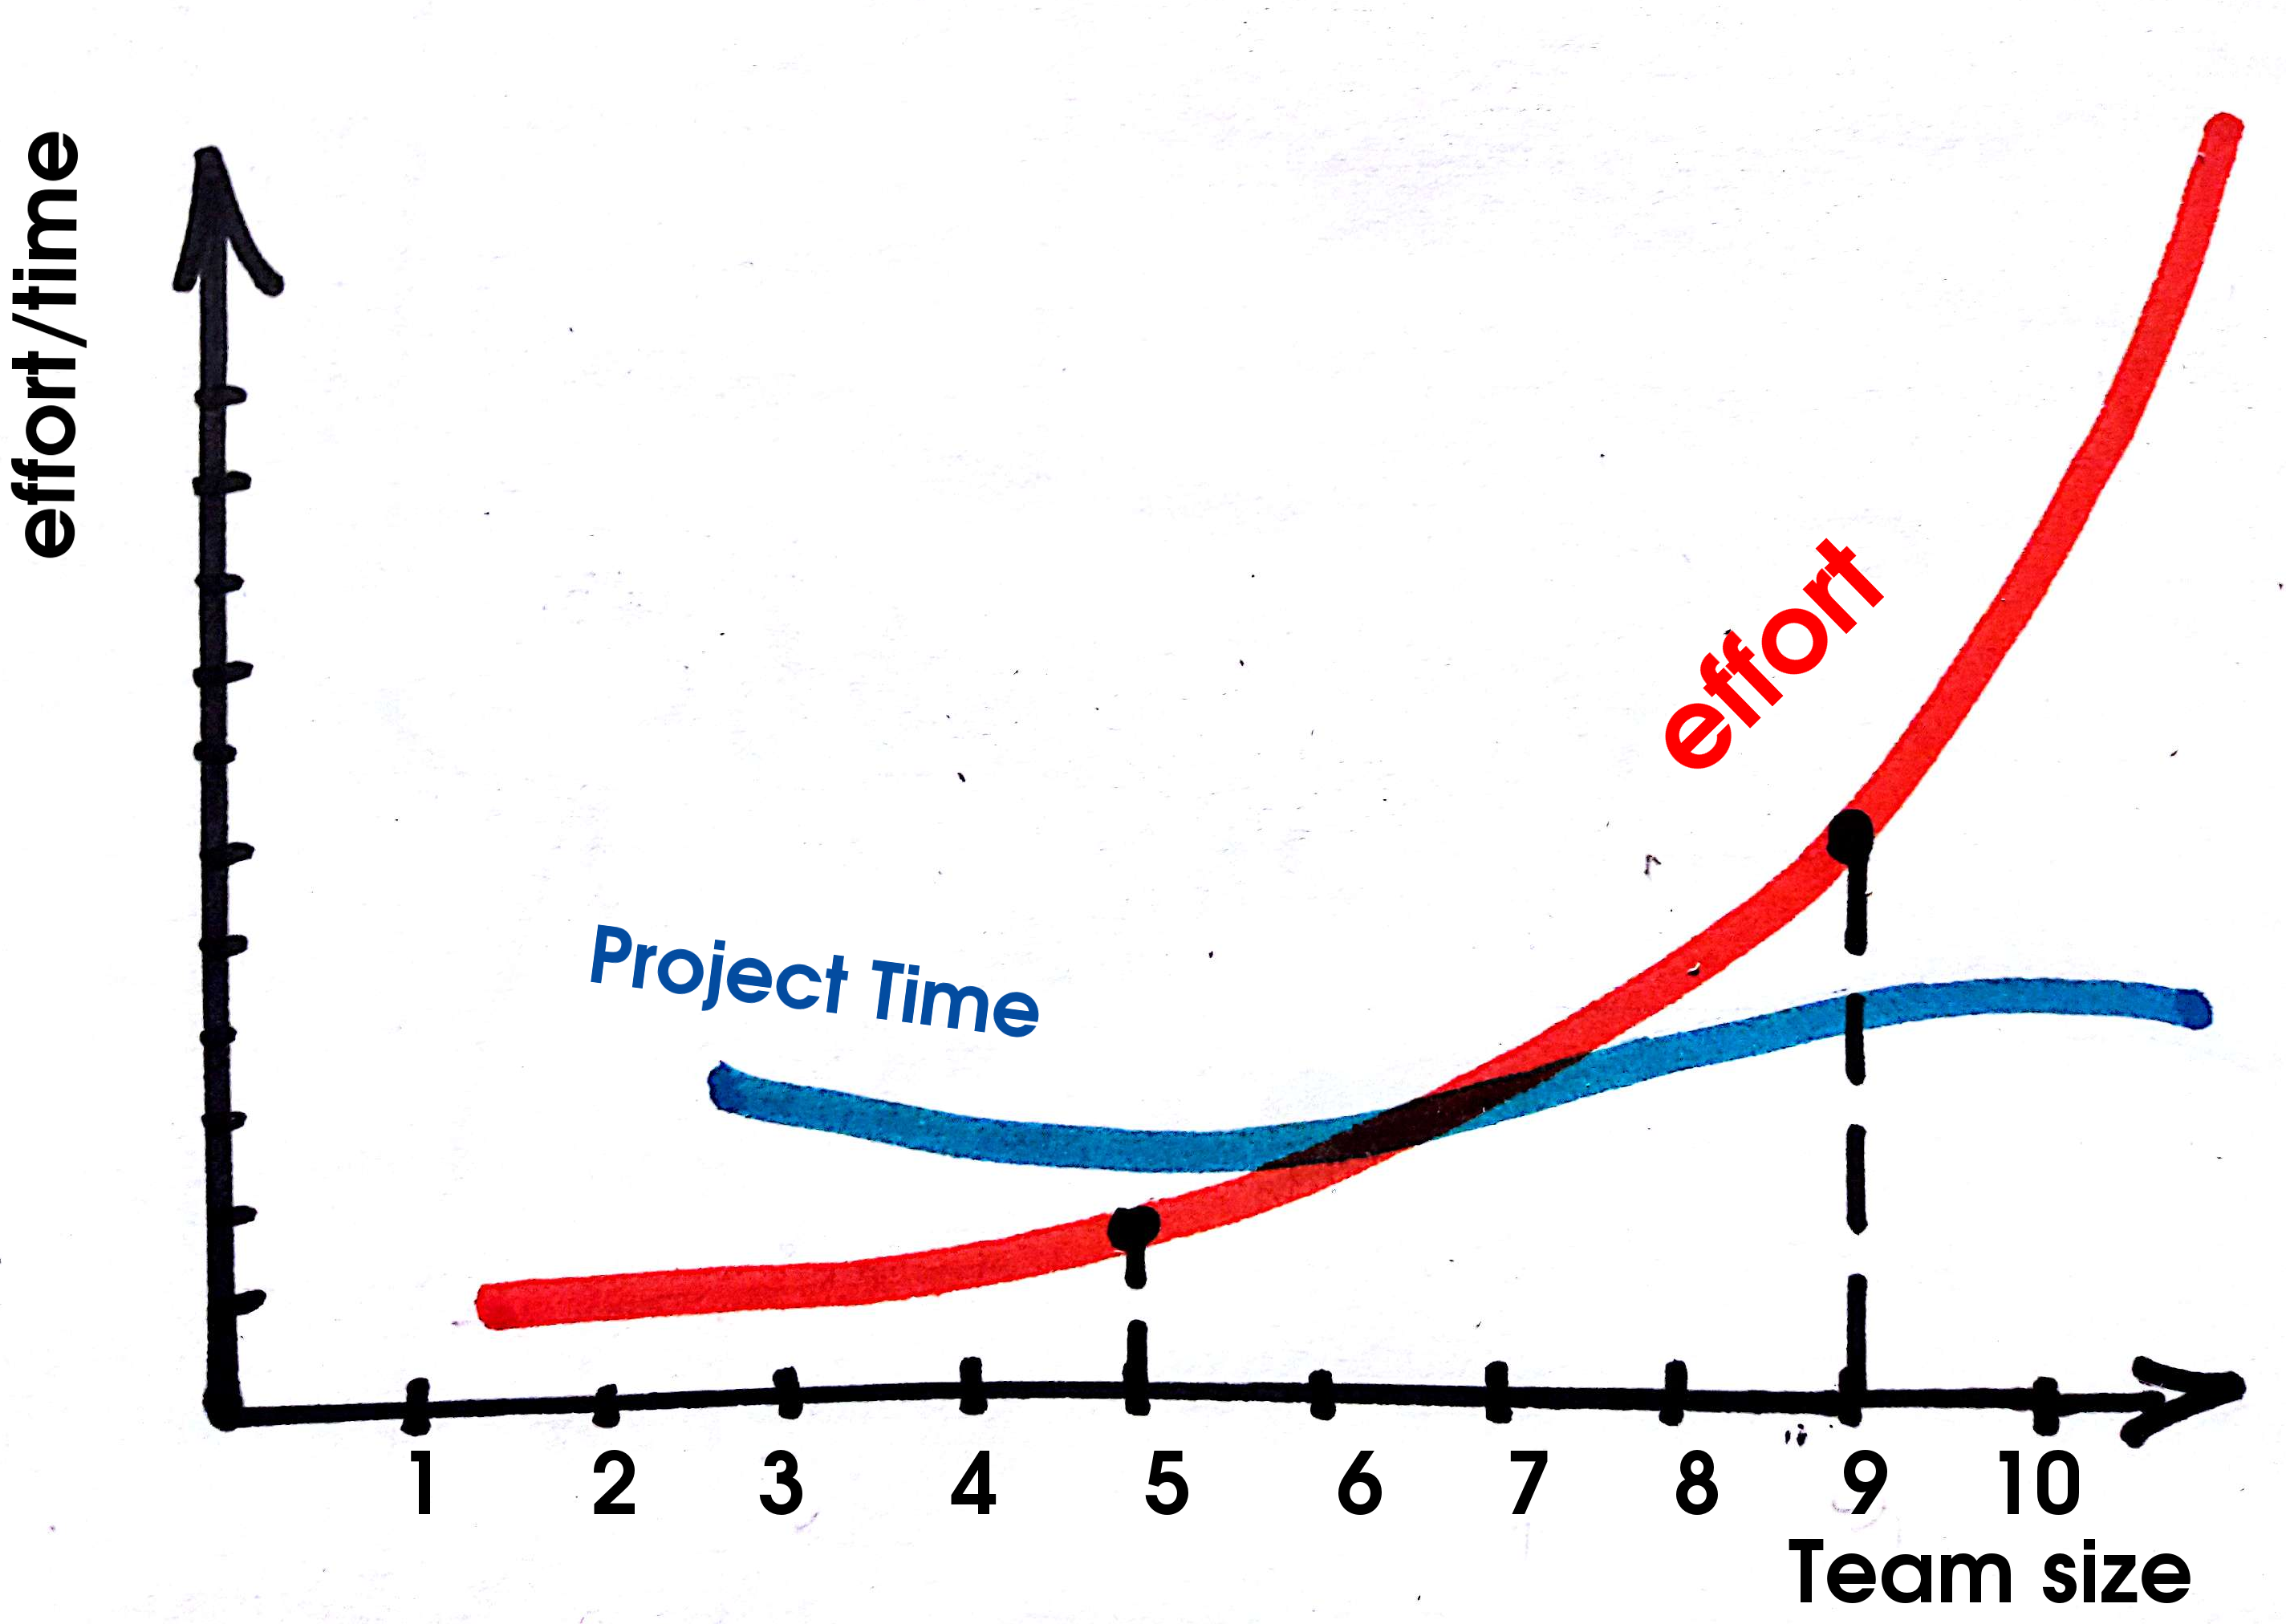
\includegraphics[width=0.60\textwidth]{TeamSize_by_Lawrence_Putnam}
  \caption{Tamaño de equipo óptimo según Putnam.}
  \centering
  \label{fig:TeamSize_by_Lawrence_Putnam} 
\end{figure}

\begin{figure}[h]
  \centering
  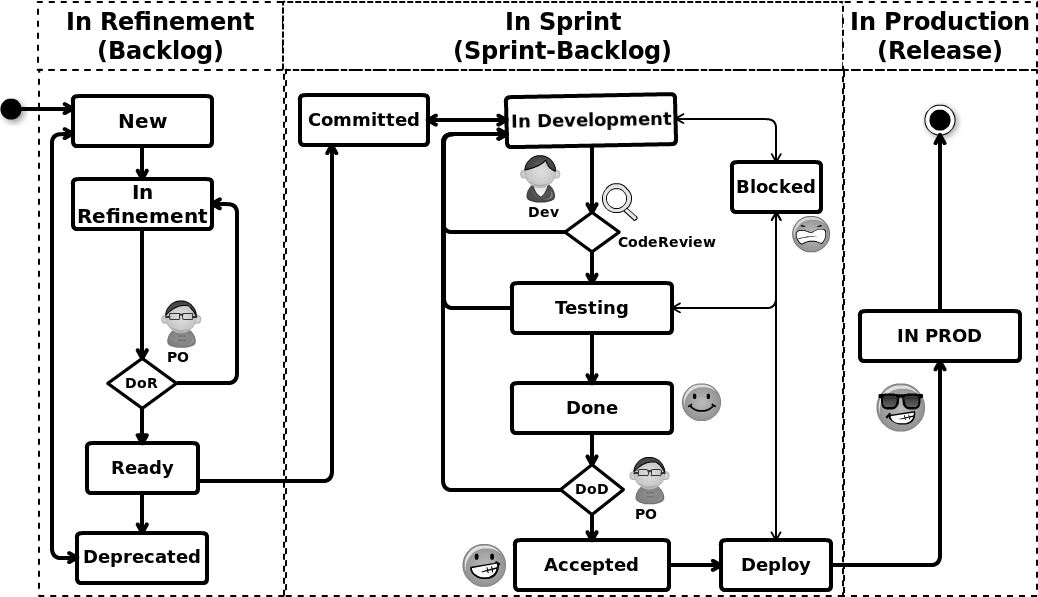
\includegraphics[width=0.99\textwidth]{StoryForkflow-Flowchart_BW}
  \caption{Diagrama de flujo de estados de un PBI o historia en el flujo de trabajo de desarrollo de software (ejemplo)}
  \centering
  \label{fig:StoryForkflow-Flowchart_BW} 
\end{figure}
